% 2.5
\subsection{質問学習モデル}
質問学習モデルはAngluin\cite{angluin-ml1988}により提案された計算論的学習理論における機械学習モデルの一つである.質問学習モデルにおいては,学習対象に関する質問に正しく答えることができる完全な教師を仮定する.この教師の役割は,現実的には実現するのが難しい状況が多く,その意味で\textbf{オラクル(oracle)}と呼ぶ.学習対象に関する質問に対して,オラクルを仮定して計算量などの解析を行う.

質問学習モデルにおいて最もよく用いられる質問として所属性質問と等価性質問がある.学習対象の概念$C$に関する所属性質問とは「任意に与えられた要素$x$が$C$に属するか否か」を問い,$Yes$か$No$のどちらかで答えを受け取る質問である(図\ref{fig:ql}).等価性質問は,学習の過程で生徒が仮説$G$を見つけたとするとき,「$G$は正しい学習対象$C$と等しいですか?」と問い,もし等しければ$Yes$と,そうでなければその反例をひとつ受け取る質問である.

% 図2.6
\begin{figure}[tb]
  \centering
  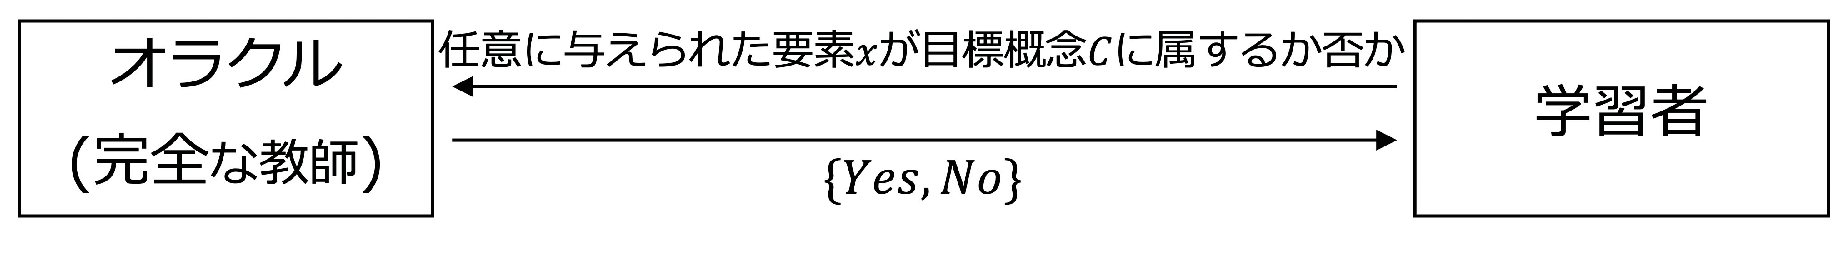
\includegraphics[scale=0.28]{fig/fig-ql.eps}
  \caption{一般に学習対象の概念$C$に関する所属性質問}\label{fig:ql}
\end{figure}